\section{Plant ROM Modeling}
\label{sec:plantRomModeling}
An issue related to the model shown in Fig.~\ref{fig:ensembleModel} is that the overall 
computation time can be very high (about 10 hours) if the outcome of each of the six 
models (i.e., PWRs and SFPs) is determined using RELAP5-3D.
Since the scope of our PRA analysis is to generate a large number number of scenarios
the computational time of the RISMC analysis would be too large even for modern high 
performance computing systems.

In order to decrease such computational time, we have employed ROMs instead of running 
the RELAP5-3D model. The objective is to employ a ROM for each PWR and SFP shown in 
Fig.~\ref{fig:ensembleModel} instead the actual code.

The actual workflow that implement such objective is as follows:
\begin{enumerate}
  \item Sample the response of each PWR and SFP using the RELAP5-3D code
  \item Choose an appropriate ROM and train it using the data generated in Step 1
  \item Validate the response of the ROMs against the response of the actual code
  \item Insert the validated ROMs in the ensemble model in place of the RELAP5-3D 
        code for each PWR and SFP
\end{enumerate}

\newcommand{\DPM}[1]{\textcolor{magenta}{#1}}

For the six plant models considered in this analysis, we have chosen to use $k$-nearest neighbor classifiers as surrogates to predict the presence of core damage in each of the models.
%
The $k$-nearest neighbor classifier is able to classify unobserved samples by employing a weighted voting system over the input space of the model.
%
In this process, first a set of observed training samples, $\mathcal{T}$, are classified according to our ground truth model.
%
In order to predict the class label of an unobserved query point, $q_i$, the $k$ \emph{nearest} samples in $\mathcal{T}$, which we will denote as $p_{i,1}$,...,$p_{i,k}$, are identified.
%
Each of the $k$ neighbors is assigned a weight and votes for its observed label.
%
The weight of the vote for $p_{i,j}$ is given by the inverse Euclidean distance between $q_i$ and $p_{i,j}$.
%
Similarly, we define ``nearest'' in terms of Euclidean or $L^2$ distance on the input space of the model being trained.

Each surrogate is trained on a separate set of Monte Carlo samples, and cross-validated using 3-fold validation in order to select an optimal value for $k$.
%
In 3-fold validation, the data is split into three roughly equal subsets and trained on two of the subsets where the third subset is used to evaluate the prediction accuracy.
%
The $k$-value that fits the data with the highest accuracy is considered the ``best'' parameter setting.
%
In order to achieve a stable optimum, we randomly select half of the training data and perform 3-fold validation over multiple iterations.
%
The results are collected into a histogram similar to Figure~\ref{fig:neighborSelection} and the most frequent ``best'' parameter is selected for $k$.
%
The values of $k$ considered are the multiple of 5 up to and including 50 (i.e., $5,10,15,20,25,30,35,40,45,50$).
%
As we can see in Figure~\ref{fig:neighborSelection}, $k=25$ most frequently reports the highest prediction classification for the held-out data for the PWR2 model and is thus reported as the optimal value in Table~\ref{tab:romInfo}.

\begin{figure}[!htbp]
	\centering
	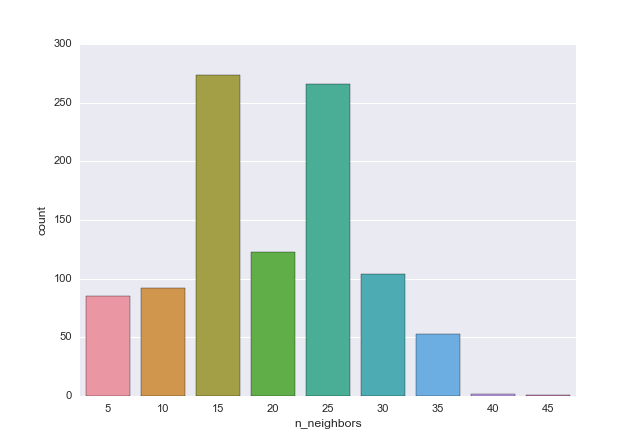
\includegraphics[width=0.98\textwidth]{neighborCVPWR2.png}
	\caption{Histogram of the ``best'' $k$ value for the PWR2 model when repeatedly trained on 500 variations of samples drawn from a pool of 4951 training samples. The training size for each instance was 2475.}
	\label{fig:neighborSelection}
\end{figure}

In order to report on the stability and convergence of each ROM, we evaluate the prediction accuracy of each ROM over increasing training sizes.
%
To this end, we compute the mean and standard deviation of the prediction accuracy over 10 iterations of each training size.
%
The prediction accuracy is always computed from the entire validation set.
%
In each case, we randomly select a set of 100 training samples, train our surrogate using this subset of training data, and predict the accuracy of the entire validation set.
%
We repeat this process ten times using a different set of randomly selected training samples and compute the mean and standard deviation for this training size.
%
Next, we add 100 training samples and repeat the entire process.
%
The process is repeated until the full training set is used.
%
Note, in the case where the full training set is used, the standard deviation will be zero since every trial of randomly selected samples will be represent the full training set.
%
This final accuracy value is the prediction accuracy reported in Table~\ref{tab:romInfo}.
%
An example of this convergence is shown in Figure~\ref{fig:romConvergence}.

\begin{figure}[!htbp]
	\centering
	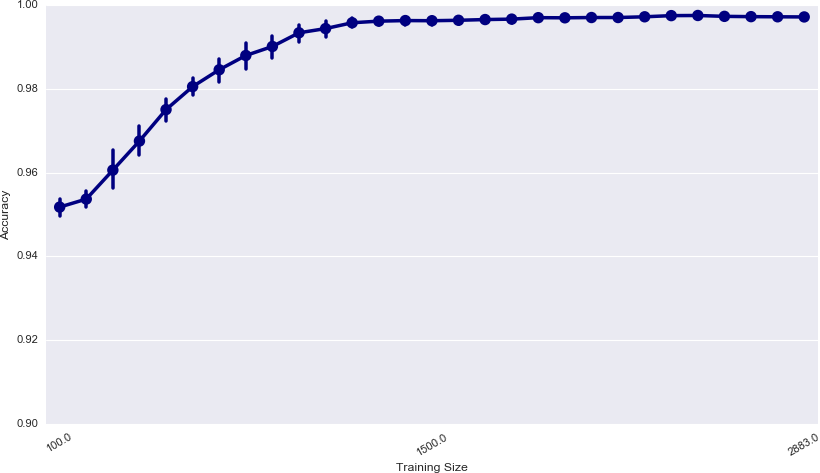
\includegraphics[width=0.98\textwidth]{convergenceSFP1.png}
	\caption{Convergence of the Prediction Accuracy with increasing sample sizes for the SFP1 model. Each data point is the average of ten trials
	worth of data with error bars representing one standard deviation. For this dataset the full training pool consists of 2883 points and accuracy is tested on an independent validation set of 2876 samples.}
	\label{fig:romConvergence}
\end{figure}

As we can see, the results are both highly stable and highly accurate.
%
The stability and precision of the results are exhibited by the presence of small error bars and a steady, gradual improvement as the size increases.
%
There are no large spikes or dips in the plot.
%
In terms of accuracy, the model accuracy is never below $90\%$ even when using only 100 samples.
%
The final parameter settings and accuracies of each model trained on its full training size are given in Table~\ref{tab:romInfo}.

\begin{table}[!htbp]
	\centering
	\begin{tabular}{ l | c | c | c | c | c }
	      & \textbf{Parameter} & \textbf{Optimal} & \textbf{Training} & \textbf{Validation} & \textbf{Prediction} \\
	\textbf{Model} & \textbf{Count}     &   \textbf{$k$}   &   \textbf{size}   &    \textbf{size}    &  \textbf{accuracy (\%)} \\
	\hline
	\hline
	PWR1 &  7 &  5 &  4596 & 2500 & 100.0 \\
	% \hline
	PWR2 &  3 & 25 &  4951 &  439 & 99.32 \\
	% \hline
	PWR3 & 10 & 50 & 12000 & 3990 & 100.0\\
	% \hline
	SFP1 &  3 &  5 &  2883 & 2876 & 99.72 \\
	% \hline
	SFP2 &  5 &  5 &  4695 & 4714 & 99.02 \\
	% \hline
	SFP3 &  3 &  5 &  2807 & 2817 & 99.04 \\
	\end{tabular}
	 \caption{Surrogate model settings and validation information.}
	 \label{tab:romInfo}
\end{table}
